% TODO:
% - Draw up a sketch of what is MIxT and what is Kvik
% - What interfaces does Kvik provide?
% - Spark, look at their papers and the app / abstractions.
% - What are the ops done most frequent? Get data from KEGG/Msigdb etc?
% - Scrap hard line breaks for LA (soft lines instead)
% - add pdf to git.

\section*{Background}
% Snakk litt om de forskjellige systemene i hver disciplin
% --> Standing on the shoulders of giants
% Analysis frameworks: R, Bioconductor, Galaxy
% Visualization: Cytoscape, BioJS, D3
% Databases: MSiGDB, KEGG, GeneCards, PubMed
% Reproducibility: Docker, R Packages, Kube
% Parallelized and distributed computation: Hadoop, Spark, Kubernets, Azure

% Analysis frameworks: Bioconductor in R, Python.
% Visualization: Cytoscpape, D3, BioJS.
% Databases: MSigDB, KEGG, PubMed.
%
% Data wrangling and analysis done in R or other languages.
% Visualization and presentation of final datasets by external tools.
% Manual database lookup is tedious and gets out of date.
%
% Related work: OpenCPU, biogo, renjin,

% LAB: overodnet, så er det en grei intro i Kvik Framework, så den kan kanskje
% modifiseres hvis ikke det er en helt annen vinkling i dette paperet

% LAB: forlag til struktur i Intro:
%
% 1. Jeg ville begynt med å beskrive "explorative data analysis" for å tolke
%  eksperiment data. Motiver behovet for visualisering + statistisk analyse +
%  referenase databaser. Jeg tror §1 og §2 fra "Kvik Framework.docx" kan brukes
%  som utgangspunkt (men med System Epidemiology fjernet). Konklusjon: det er
%  stort behov for slike verktøy.
%
% BF: Tror det her egentlig er mer snakk om tolkning av resultater enn
% 'explorative data analysis'. Hvertfall i mitt hode er 'explorative data
% analysis' noe man gjør i R, man laster inn data, prøver ut forskjellige typer
% analyser og ser hvordan ting ser ut. Dette er ikke nødvendigvis det vi trenger
% Kvik til. Kvik kan brukes når man allerede har plugget inn dataen sin, og
% prøvd ut noen ting før man vil dele det med andre. 

% 2. Deretter ville jeg beskrevet behovet for å lage spesialiserte data
%  exploration verktøy. Jeg tror "Such special purpose..." § fra Framwork kan
%  omskrives. Konklusjon: det er behov for å raskt kunne skrive exploration apps
%  prototyper. Reviwerene av app note likte dette poenget, og i mitt hode er
%  dette hoved målet/bidraget i dette paperet.
%
% BF: Enig. Man kan jo egentlig tenke litt på det som en iPython Notebook / R
% Notebook, bare som er skikkelig verktøy. 
% BF: Et poeng med måten jeg har valgt å bygge Kvik er at man kan skrive seg en
% R-pakke som man gjør når man gjør analyser, og så kan man ta den med seg inn i
% nettleseren for å vise fram det man har gjort + koble sammen med andre greier. 

% 3. Jeg er usikker på om vi skal argumentere for at det ofte blir behov for å
%   skalere/ optimalisere/ deploye de prototype appene. Det passer kanskje godt
%   med bidraget i dette paperet?
%
% BF: Tja, hvertfall at performance er viktig når det kommer til større analyser
% er jo et poeng. Vi kan jo la det ligge litt og se hva vi får ut. Når det
% kommer til hva som er gjort kan vi jo si at kvik er raskere enn opencpu. 

% 4. Requirements mener jeg er:
%    i. "JavaScript + R"
%   ii. Easy to add new functionality (viz or stat)
%  iii. Short reponse times
%   iv. Reference databases: up-to-date with provenance and space effecient storage
%    v. Integration with (big data/ distributed) data analysis and exploration engines
%   vi. Noe jeg ikke har fått med meg?

% BF: 
%   i: AnyLang + R 
%   ii. Mulighet for å installere egne/andres R-pakker 
%   iii. Fast (short response times) 
%   iv: up-to-date reference databases
%   v: 
    

% 5. Deretter hvorfor previous work ikke løser alle 5
% 6. Hva Kvik er:
%    i. Lag mellom viz & stat & DBs (merk usikker på hvor input/output data passer inn)
%
%            JavaScript (Visualization)
%                        ||
% Inpup/output data? == KVIK == Reference databases
%                     //   \\
% R (Statistical analysis)  Other engines (scale/speed)


%  ii. Abstraksjoner/ interfaces som gjør det raskt å protype exploration apps
%  iii/v. En slags execution engine som router requests til rett sted. Dvs den
%  tilbyr funksjonalitet i seg selv (ikke sikker på hva dette er :) 
% BF: Denne må
%  du fortelle meg hva er, skjønner ikke helt her. 

%  iv. Caching, logging, etc. Dette er en viktig bit vil jeg tro, særlig når ref
%  DBs begynner å bli veldig store.
% BF: Yes, det som er på plass nå er caching av alt av DB requests (om jeg ikke
%   husker feil) 

% 7. Contributions:
%  i. Approach for vis + stat + DB m. enkel implementering
%  ii. Demonstrasjon ved å ha implementert 3-4 apps
%  iii. Performance evaluation

In the past decade the generation of biological datasets has been unprecedented,
and the famous "\$1000k genome, \$1M analysis"\cite{} has become more apparent.
To decrease both time and cost of analysing biological data, there is now a
growing number of analysis framework in various programming languages.\cite{}

In R, there are popular package repositories such as CRAN
\url{cran.r-project.org} or Bioconductor \url{bioconductor.org} where developers
can share software packages and keep them up-to-date. In these repositories
researchers can find software for analysing high-throughput genomic data in one
environment. Analysing includes both pre-processing, e.g. cleaning, removing
outliers, and analysing it with known statistical methods.

Interpreting the analysis results require integration of known biology, either
from biological databases such as MSigDB\cite{} or KEGG\cite{}, or through
scientific publications from databases such as PubMed\cite{}. Performing manual
lookup into these databases is often tedious and error-prone, making it
necessary to automate the task. % ikke så bra avsnitt dette... 

Especially large datasets in biology require sophisticated methods for
visualizing and interpreting the results, as well as communicating and sharing
the findings.

\subsection*{Data analysis} 
In this section we describe our typical approach for doing analysing gene
expression data in systems biology, and how it shaped the design of Kvik's
R interface. 

We typically start off with a messy dataset that needs to go through
several stages of clean-up and preprocessing before we can analyze it. After the
preprocessing we typically develop some simple visualizations that can highlight
simple patterns in the data. After this quick dirty data exploration we start to
apply more advanced statistical methods to look for more intricate patterns in
the data.  After this analysis we often end up with genes or lists of genes of
interest. 

In terms of data analysis code, the preprocessing steps typically consist of
one or more R scripts that we knit \cite{knitr} into PDF reports that we can
revisit later. From these scripts we end up with analysis-ready datasets that
can be shared within the group. The remaining downstream analysis often starts
out in scripts, that are built into R packages with analysis code that can be
shared between researchers. 

With this process in mind, we designed the interface to the R programming
language in Kvik. We want to make it possible to call any function from an R
package and return its results either as plain text, such as comma-separated
tables, or binaries such as images. Enforcing that R code is built into R
packages ensures that the analysis code can be used by power users through an
ordinary R session or in the data exploration application itself. 


\subsection*{Databases} 
Similar to how our analysis process shaped the R interface, it also defined how
we want to build interfaces to online databases. 

In its initial state we wanted an interface to interactively query databases
such as KEGG or MSigDB for up-to-date information about genes, gene sets or
biological pathways. This interface should be available within the data
exploration applications to provide valuable metadata for the researchers
exploring results.  

\subsection*{Building applications} 
With Kvik there are multiple aveues developers can take to build data
exploration applications. They can choose to develop a single tiered
applications with bindings to data analysis and databases, or
multitier architectures where data analysis can be moved to powerful compute
clusters to improve performance. In this paper we discuss how to develop
applications that follow a multitier architecture. 

In Kvik we use R packages as the fundamental building block for data exploration
applications. They provide an interface to data and analyses, and especially in
the field of systems biology, the R programming language provide the largest
collection of data analysis packages. % litt vagt kanskje? 
We discovered that the most sensible way to build applications on top of our
existing code base was to build a system that could interface with our analysis
code directly. 

Applications built with Kvik start out as R packages where the functions provide
interface between the data and 

for the application. 



\subsubsection*{Requirements} 
\begin{enumerate}
    \item A language-independent approach for integrating statistical software,
    such as R, directly in interactive data exploration applications.
    \item Up-to-date interfaces to online databases providing meta-data for
    understanding results from statistical analyses. 
\end{enumerate} 

\subsubsection*{Contributions} 
Our contributions are: 
\begin{enumerate}
\item An approach for developing data exploration applications in systems
biology that combine statistical analyses with online databases.  
\item A demonstration of its viability through N different applications. 
\item Performance evaluation of its central data analysis component. 
\end{enumerate} 


% The big issue: There is no link between analysis and final presentation

\subsection*{Motivating example}

% MIxT.
% Interactive web application for exploring WGCNA modules from blood and biopsy.
% Integrate results with known genesets and online databases.
% Docker containers for reproducibility and portability.
% Data analysis: R package  + Kvik = R in the browser.
% Visualization: D3, SigmaJS, R Plots
% How can we improve Kvik and its features: R user input sanitation, security,

% Data analyse og livet: 
% Det som oftest gjøres er at man skriver et R-scriot

We motivate the need for Kvik by describing the MIxT application for exploring
and comparing transcriptional profiles from blood and tumor samples. We
describe its functionality, implementation 
% (uten fokus på Kvik)
and performance requirements.
%OG ANDRE VIKTIGE TING (SECURITY, ETC). 
Then we describe how MIxT
is designed to separate concerns and allow for a layered implementation. We use
this to motivate the need and opportunities to abstract away common
functionality of these type of applications.

% Det kan godt være at vi bør flytte denne et sted, men her beskriver vi hvordan 
% MIxT-appen fungerer. 
\subsection*{Matched Interaction Across Tissues (MIxT)}
We have built a system to identify genes and pathways in the primary tumor that
are tightly linked to genes and pathways in the patient systemic
response\cite{dumeaux2017}. MIxT blood-tumor is an open-source web application
for exploring the molecular processes expressed in each tissue.  

For the web application we defined six analysis tasks: 

\textbf{Explore co-expression relationships between genes}. Create an
interactive network visualization that visualizes each gene as a node and
significan co-expression relationship as an edge. 

\textbf{Explore co-expression gene sets in tumor and blood tissue}.
Visualize gene expression together with clinicopathological variables associated
with each module. Include results of gene set analyses that describe the
underlying biological functions of the modules. 

\textbf{Explore relationships between modules from each tissue.}
Visualize how modules from each tissue are related using two different
metrics, ranksum and gene overlap. Also enable subtype selection,
enabling users to investigate relationships within a particular subtype. 

\textbf{Explore relationships between clinical variables and modules.}
Visualize significant associations between module expression and
clinical variables.

\textbf{Explore association between user-submitted gene lists and computed
modules.} Allow users to upload own gene lists and have the application compute
modules which the gene list is enriched for. 

\textbf{Search for genes or gene lists of intrest.} Allow users to search
for specific genes or genelists and show 

% Vi kan godt kutte én av figurene under, f.eks c eller d som er veldig lik. 
\begin{figure*}[!t]
\centering
\subfloat[A1: Network visualization of gene
co-expression]{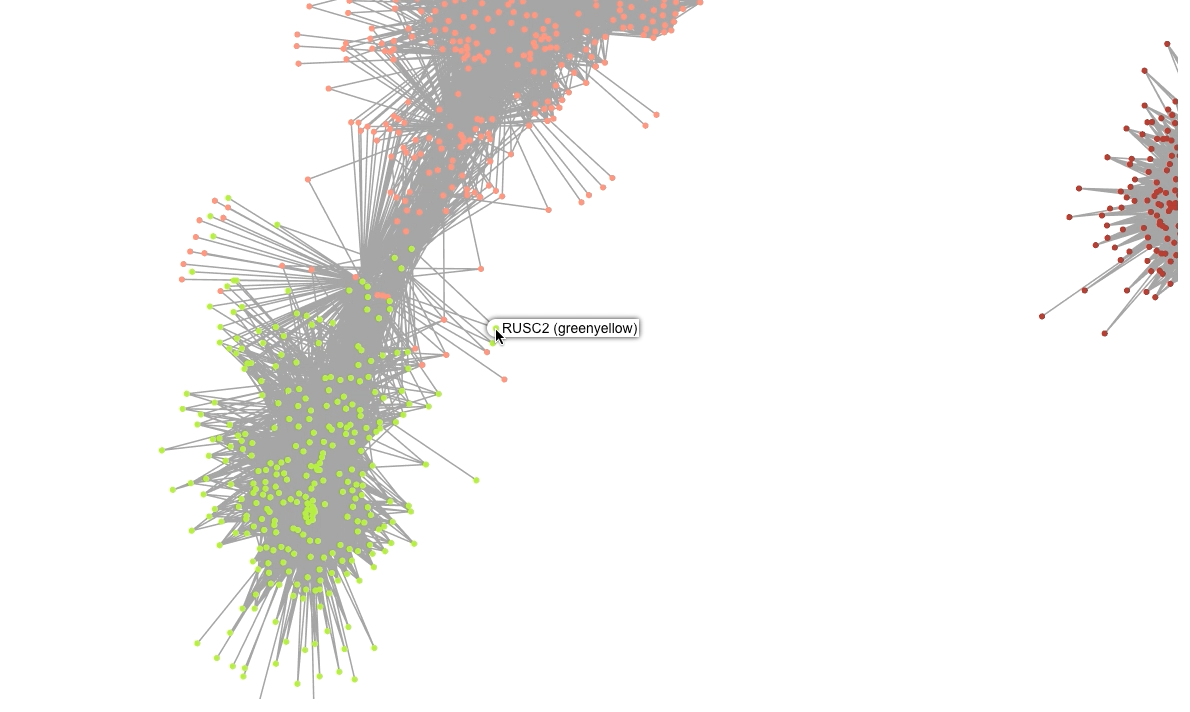
\includegraphics[width=2.7in]{figures/network.png}%
\label{fig_first_case}}
\hfil
\subfloat[A2: Module visualization.]{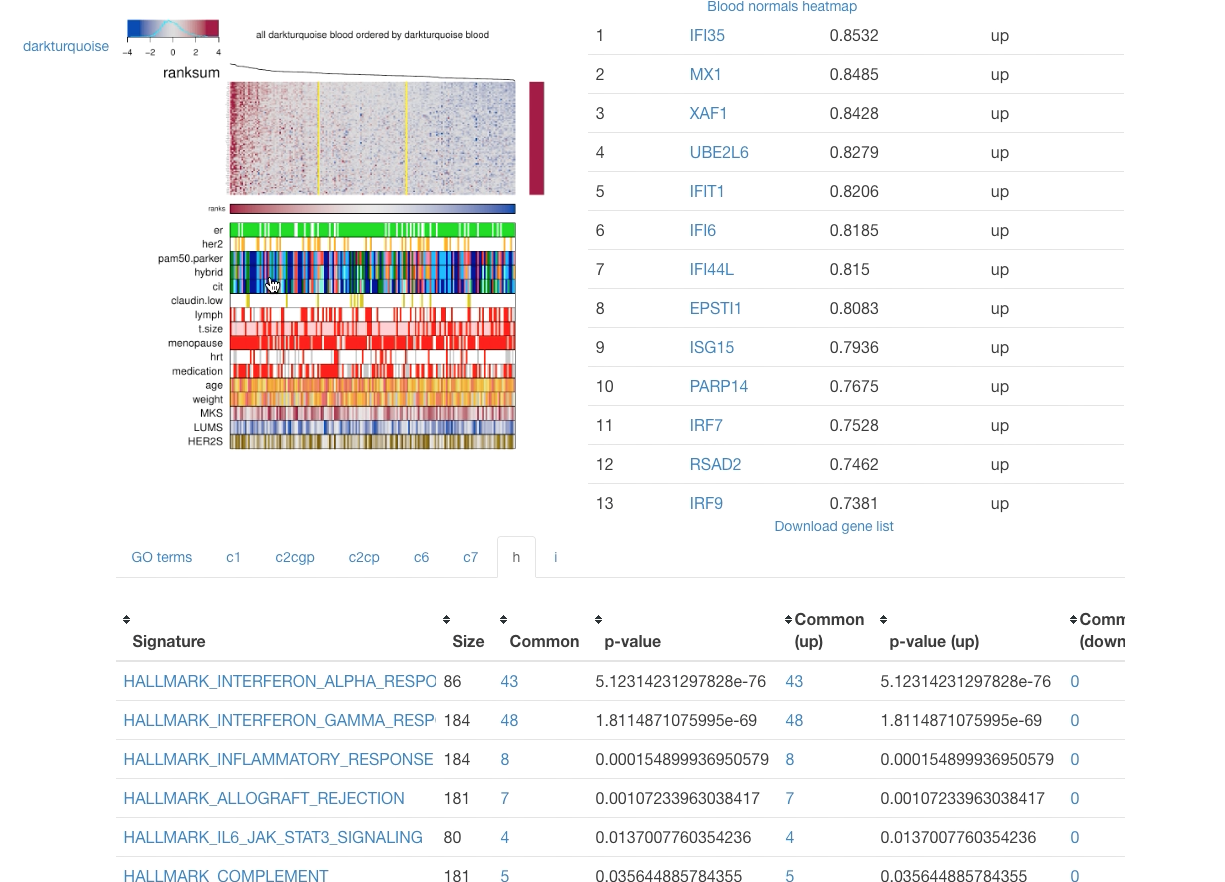
\includegraphics[width=2.5in]{figures/module.png}%
\label{fig_second_case}}
\hfil
\centering
\subfloat[A3: Visualization of ranksum.]{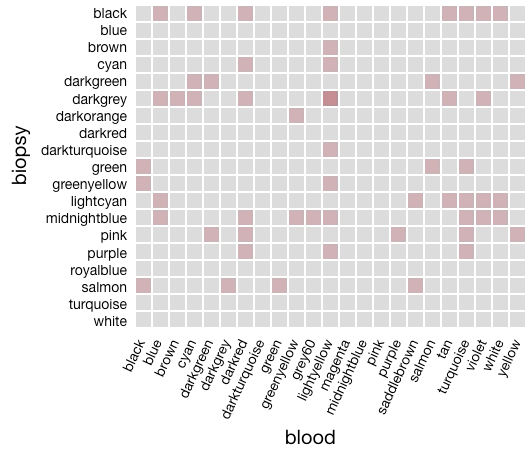
\includegraphics[width=2.5in]{figures/tissue-comp.png}%
\label{fig_first_case}}
\hfil
\subfloat[A4: Visualization of significant clinical variable
association]{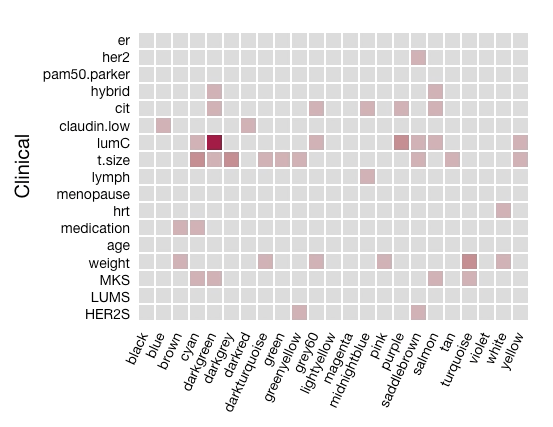
\includegraphics[width=2.8in]{figures/clinical-comp.png}%
\label{fig_second_case}}
\caption{Screenshots of the user interface in four of the six analysis tasks.
Note that we combine visualization frameworks for both JavaScript and R to
generate the visualizations. Specifically,
sigmajs (a, \protect\url{sigmajs.org}), ggplot2(b, \protect\url{ggplot2.org}), and 
D3 (c and d, \protect\url{d3js.org})} 
\label{fig_sim}
\end{figure*}




% Gir dette mening?

\section*{Methods}
% Collection of packages in the Go programming language for building data
% exploration applications.  Interfaces with popular online databases such as
% MSigDB and KEGG.  Provides an interface to the R programming language.
% Typically used to build web apps, but commandline tools are also possible!

% LAB: denne bør begynne med Architecture/overview: ASCII figuren fra Intro, kanskje litt rafinert:
%  * Interface mot JavaScript er en mer generell REST API, så kan være cli eller noe annet som bruker den.
%  * Reference databases er kanskje en egen "ting" i Kvik. Dvs abstraksjoner som gjør det enkelt å implementere disse for MSigDB, KEGG. Dvs de tar seg av caching og provenance.
%
% Her passer det også å vise hvordan MIxT mappes til figuren. 

% LAB: jeg tenker på dette som en slags execution engine, og at dette er laget mellom R og JS. 
% Hva slags interface exporter den til JS? Og hvorfor?
% Hva gjør den? Og hvorfor kan ikke dette gjøres i JS eller R?
% Hva er det som er generelt? Og hva er app spesifikt?
% Hva er gjort for å få god performance?
% Andre ting denne tar seg av?
% Hvorfor, og hvordan, det er lett å legge til ny funksjonalitet
\subsection*{Statistical analyses}
Describe how we've designed the interface with R: Build an R-package and call
functions from it, we provide four different output formats to the user
 (json, csv, pdf, png),  as well as four different http endpoints (call, get and
rpc).

% LAB: jeg tenker på dette som en måte å implementere støtte for ulike refDBs. Dvs den tilbyr abstraksjoner/ data strukturer/ wrappere/ metoder for:
% * Hente data fra online DBs (feilhåndtering, etc)
% * Caching av data hentet fra online DBs
% * Provenance logging / managemnt for data fra online DBs
% * En måte å effektivt lagre disse DB på, både for god performance og lite space
% * En måte å gjenbruke kode (og data) for en DB som feks KEGG
% * Eventuelt andre ting denne tar seg av?
%
% I tillegg:
% Hvorfor ikke gjøre dette i JS eller R?
% Hvordan implementerer man KEGG etc?
\subsection*{Databases}
Describe the interface to the databases and what we use it for. Could be
interesting to talk about provenance/caching.

% LAB: her er stedet for alle Go bibliotek og andre lavnivå detlajer
\subsection*{Implementation}

% LAB: Litt usikker på om dette hører til i Results eller Methods
\subsection*{Applications}

% LAB: kort beskrivelse av hva alle apps gjør

% LAB: Figur som viser hva som er felles og ulikt for alle appene. Her bør noe være likt ellers har vi bare 3-4 applikasjoner :)

% LAB: mer detaljert beskrivelse av hvordan hver app er implementert med Kvik

\section*{Results and Discussion}
Describe the MIxT application. Also talk about how our R interface scales and
what makes it better than opencpu/renji.

% LAB: Questions:
% 1. Er execution engine raskere en andre alternativer? Svar: måle mot andre alternativer.
% 2. Gir ref DB caching bedre performance? Svar: som i master thesis.
% 3. Har provenance mangement høy overhead (response tid & storage)? Svar: måle disse.
% 4. Er det lett å legge til ny funksjonalitet (viz & stat & optimizations)? Svar: beskrive hvordan ikke-MIxT apps ble laget
% 5. Er Kvik apps raske? Svar: performance analyze av MiXT, inkl. bottlenecks, skalerbarhet, etc.
% 6. Er Kvik apps enkle å utvikle/vedlikeholde? Svar: beskrive hvordan MiXT ble laget (fra mess til den vakre nåværende kodebasen).

\section*{Conclusions}
